\documentclass[12pt,a4paper]{article}
\usepackage{cmap}
\usepackage[utf8]{inputenc}
\usepackage[T1,T2A]{fontenc}
\usepackage[english,russian]{babel}
\usepackage{array,booktabs,tabularx,amsmath}
\usepackage{caption,float,graphicx,qrcode}
\usepackage{geometry,hyperref,indentfirst}
\geometry{margin=25mm}
\hypersetup{unicode=true,colorlinks=true,urlcolor=blue,linkcolor=black}
\setlength{\parindent}{1.25cm}
\setlength{\parskip}{0pt}
\setlength{\emergencystretch}{2em}
\renewcommand{\labelitemi}{\textendash}
\DeclareCaptionLabelSeparator{emdash}{\space---\space}
\captionsetup[figure]{justification=centering,singlelinecheck=false,labelsep=emdash}
\addto\captionsrussian{\renewcommand{\figurename}{Рис.}}
\newcommand{\ZipfDate}{07.11.2026}
\newcommand{\ZipfDocuments}{478\,833}
\newcommand{\ZipfBytesMB}{1\,439,91}
\newcommand{\ZipfTokens}{158\,544\,765}
\newcommand{\ZipfVocabulary}{1\,451\,704}
\newcommand{\ZipfHapax}{715\,896}
\newcommand{\ZipfHapaxPercent}{49,31}
\newcommand{\ZipfSeconds}{123,66}
\newcommand{\ZipfMemory}{64}
\newcommand{\ZipfAlpha}{1,0098}
\newcommand{\ZipfFitMin}{10}
\newcommand{\ZipfFitMax}{10\,000}
\newcommand{\ZipfCountingRuns}{19}
\newcommand{\ZipfRankingRuns}{8}
\newcommand{\ZipfTitleOnly}{6\,514}
\newcommand{\ZipfRuAlpha}{0,970}
\newcommand{\ZipfEnAlpha}{1,197}
\newcommand{\ZipfGroupRows}{%
Весь корпус & 478\,833 & 158\,544\,765 & 1\,451\,704 & 1,010 \\
EN-источники & 150\,936 & 76\,281\,373 & 476\,352 & 1,197 \\
RU-источники & 327\,897 & 82\,263\,392 & 1\,071\,670 & 0,970 \\
Eurogamer & 77\,772 & 39\,683\,597 & 307\,718 & 1,192 \\
GameMAG & 73\,772 & 13\,353\,009 & 364\,833 & 1,011 \\
GamingOnLinux & 28\,184 & 9\,807\,109 & 110\,486 & 1,313 \\
Игромания & 50\,818 & 15\,532\,575 & 448\,979 & 0,940 \\
IXBT.games & 68\,315 & 12\,414\,301 & 314\,938 & 1,007 \\
PC Gamer & 44\,980 & 26\,790\,667 & 253\,863 & 1,184 \\
PlayGround & 80\,634 & 14\,421\,804 & 357\,310 & 0,982 \\
StopGame & 54\,358 & 26\,541\,703 & 636\,802 & 0,967 \\
}

\begin{document}
\hypersetup{pageanchor=false}
\begin{titlepage}
\begin{center}
{\large МОСКОВСКИЙ АВИАЦИОННЫЙ ИНСТИТУТ\\
(НАЦИОНАЛЬНЫЙ ИССЛЕДОВАТЕЛЬСКИЙ УНИВЕРСИТЕТ)}
\vspace{18pt}
{\large Факультет информационных технологий и прикладной математики}

{\large Кафедра вычислительной математики и~программирования}
\vfill
{\large\textbf{Лабораторная работа №5 по курсу\\ «Информационный поиск»}}
\vspace{12mm}

{\large\textbf{Закон Ципфа}}
\vfill
\begin{flushright}
\begin{tabular}{@{}r@{:\hspace{0.6em}}l@{}}
\textit{Студент} & К.\,А. Арусланов\\
\textit{Группа} & М8О-403Б-23\\
\textit{Преподаватель} & А.\,А. Кухтичев\\
\textit{Дата} & \ZipfDate\\
\textit{Оценка} &
\end{tabular}
\end{flushright}
\vfill
Москва, 2026
\end{center}
\end{titlepage}
\hypersetup{pageanchor=true}
\setcounter{page}{2}
\tableofcontents
\newpage

\section{Постановка задачи}
Для своего корпуса необходимо построить график распределения терминов по
частотностям в логарифмической шкале, наложить на этот график закон Ципфа.
Объяснить причины расхождения.

\section{Метод решения}
\subsection{Корпус и единица подсчёта}
Исследуются русскоязычные и англоязычные публикации о компьютерных играх
восьми сайтов. Из MongoDB экспортирован локальный снимок из
\ZipfDocuments{} пригодных документов: \ZipfBytesMB{} МБ заголовков и
основного текста в UTF-8. \ZipfTitleOnly{} публикаций участвуют только
заголовком. Для всех измерений используется один и тот же снимок корпуса.

Единицей подсчёта является нормализованная словоформа, выделенная на этапе
токенизации. Лемматизация не применяется: например, «игра», «игры» и «игрой»
учитываются отдельно. В работе исследуется распределение словоформ.
Стоп-слова сохраняются, поскольку они составляют наиболее частую часть
лексики. Заголовки и основной текст учитываются совместно.
Частота $f$ равна общему числу вхождений термина, включая повторения
в одном документе.

\subsection{Подсчёт с ограничением памяти}
Основной алгоритм написан на C++17 без контейнеров STL и готовых структур
частотного словаря. Используются собственная хеш-таблица с линейным
пробированием и внешняя сортировка. Для каждой группы подсчитывается число
вхождений каждого термина. При заполнении выделенного буфера частоты
сортируются и сохраняются частями. Последующее слияние суммирует частоты
одинаковых терминов из разных частей.

Второй внешний проход упорядочивает пары по убыванию частоты внутри группы.
При равенстве используется лексикографическое сравнение UTF-8. Каждому
токену присваивается отдельный ранг, начиная с единицы. Весь корпус и весь
итоговый словарь не требуется хранить в оперативной памяти.
Объём буфера счётчика составляет \ZipfMemory{} МиБ; дополнительная память
используется для чтения текста и слияния частей.

\subsection{Модели и разрезы}
Пусть $N$ --- число вхождений, $V$ --- число различных терминов.
Теоретическая кривая закона Ципфа имеет вид
\[
 f_Z(r)=\frac{C}{r},\qquad C=\frac{N}{H_V},\qquad
 H_V=\sum_{r=1}^{V}\frac1r.
\]
Такая нормировка даёт сумму теоретических частот, равную $N$.
Она не обязывает значение в первой точке совпасть с частотой самого
популярного слова. В логарифмических координатах модель является прямой
с наклоном $-1$.

Дополнительно C++ подбирает $f_P(r)=C_P/r^\alpha$ линейной регрессией
$\ln f=\ln C_P-\alpha\ln r$ на рангах
\ZipfFitMin{}--\ZipfFitMax{} в пределах словаря группы. Это отдельная
оценка наклона выбранного участка распределения. При $\alpha=1$ модель
совпадает по форме с законом Ципфа. Близость показателя к единице на этом
интервале не означает совпадения распределений на всех рангах.

На графике эта кривая обозначена как аппроксимация. Для каждого ранга
выбранного интервала вводятся $x_r=\ln r$ и $y_r=\ln f_{\text{набл}}(r)$.
По этим точкам методом наименьших квадратов оценивается прямая
$y=a+bx$, то есть минимизируется
\[
\sum_{r=r_{\min}}^{r_{\max}}
\bigl(y_r-a-bx_r\bigr)^2.
\]
После оценки коэффициентов выполняется обратное преобразование:
$C_P=e^a$, $\alpha=-b$. Таким образом, по логарифму ранга оценивается
логарифм частоты, а в исходных координатах получается степенная кривая.
Аппроксимация описывает наклон выбранного участка данных. Для сравнения
с законом Ципфа отдельно используется модель с фиксированной степенью 1.

Кроме общего распределения рассчитываются группы по сайтам и языкам
источников. Язык определяется по источнику;
внутри русскоязычных публикаций могут присутствовать английские названия.

В сравнительных рисунках используется относительная частота $f/N$ каждой
группы. Иначе высота линии отражала бы прежде всего объём сайта.
Ранг и нормировка вычисляются внутри группы. Один документ участвует
в нескольких разрезах: складывать показатели между разрезами нельзя.

\subsection{Проверка корректности}
План тестирования включает контрольные корпуса с заранее известными
частотами, проверку ранжирования и группирования, а также сравнение
результатов при разных размерах буфера. Последняя проверка подтверждает,
что разбиение на части и многопроходное слияние не изменяют итоговые частоты.
Подбор показателя степени проверен на распределении $f(r)=60/r$ для
рангов 1--5, для которого ожидается $\alpha=1$. Дополнительно проверяется
обработка некорректных входных данных.

Успешно пройдены 11 C++-тестов GoogleTest, одна проверка запуска программы
и 5 тестов подготовки данных, сравнения и графиков. На полном корпусе проверено,
что сумма частот равна числу учтённых токенов, а суммы по сайтам
и языкам согласуются с общими показателями. Журнал проверок
приложен в \path{lab5/tests.txt}.

\section{Результаты}
\subsection{Общая статистика}
\begin{table}[H]
\centering
\begin{tabularx}{\linewidth}{@{}Xr@{}}
\toprule
Показатель & Значение\\
\midrule
Документы & \ZipfDocuments\\
Токены $N$ & \ZipfTokens\\
Различные термины $V$ & \ZipfVocabulary\\
Термины с одним вхождением (hapax) & \ZipfHapax\\
Доля hapax в словаре, \% & \ZipfHapaxPercent\\
Подобранная степень $\alpha$ & \ZipfAlpha\\
Время C++ с чтением и записью, с & \ZipfSeconds\\
\bottomrule
\end{tabularx}
\end{table}

Измерение выполнено для Windows Release-сборки GCC 13.1.0.
Приведено время одного запуска с чтением корпуса и записью частот;
экспорт данных и построение графиков не учитываются. Использовался
прогретый файловый кеш.

\begin{figure}[H]
\centering
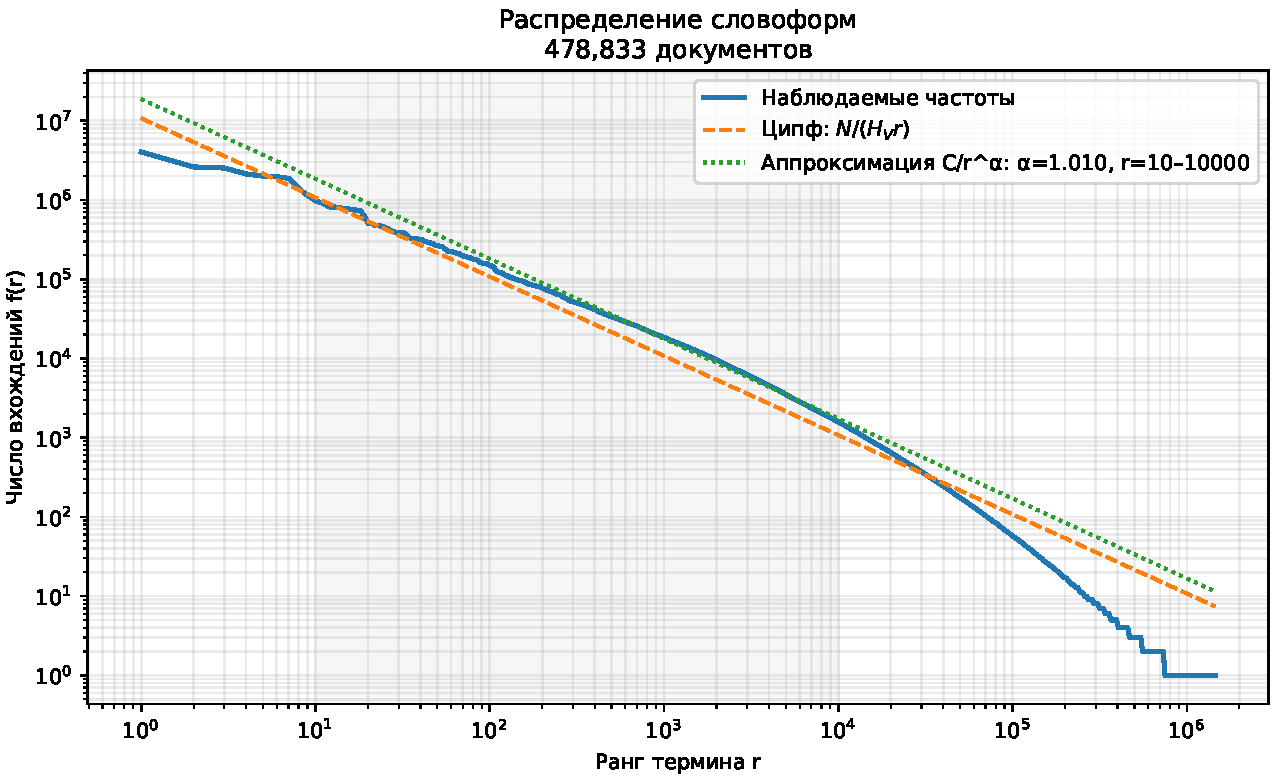
\includegraphics[width=\linewidth]{lab5/zipf_all.pdf}
\caption{Наблюдаемые частоты, закон Ципфа и аппроксимация; серым выделен интервал оценки степени}
\end{figure}

На средних рангах распределение близко к прямой, а подобранное
$\alpha=\ZipfAlpha{}$ близко к единице. Однако в начале кривой и в хвосте
наблюдаются отклонения. Почти половина словаря встречается один раз;
частоты 1, 2 и 3 образуют ступени, а не гладкую прямую. Число hapax
не следует интерпретировать как число опечаток: сюда входят редкие имена,
названия, словоформы и нормальные малочастотные слова.

\subsection{Сравнение источников и языковых групп}
\begin{table}[H]
\centering
\small
\begin{tabularx}{\linewidth}{@{}Xrrrr@{}}
\toprule
Группа & Документы & Токены & Словарь & $\alpha$\\
\midrule
\ZipfGroupRows
\bottomrule
\end{tabularx}
\end{table}

\begin{figure}[H]
\centering
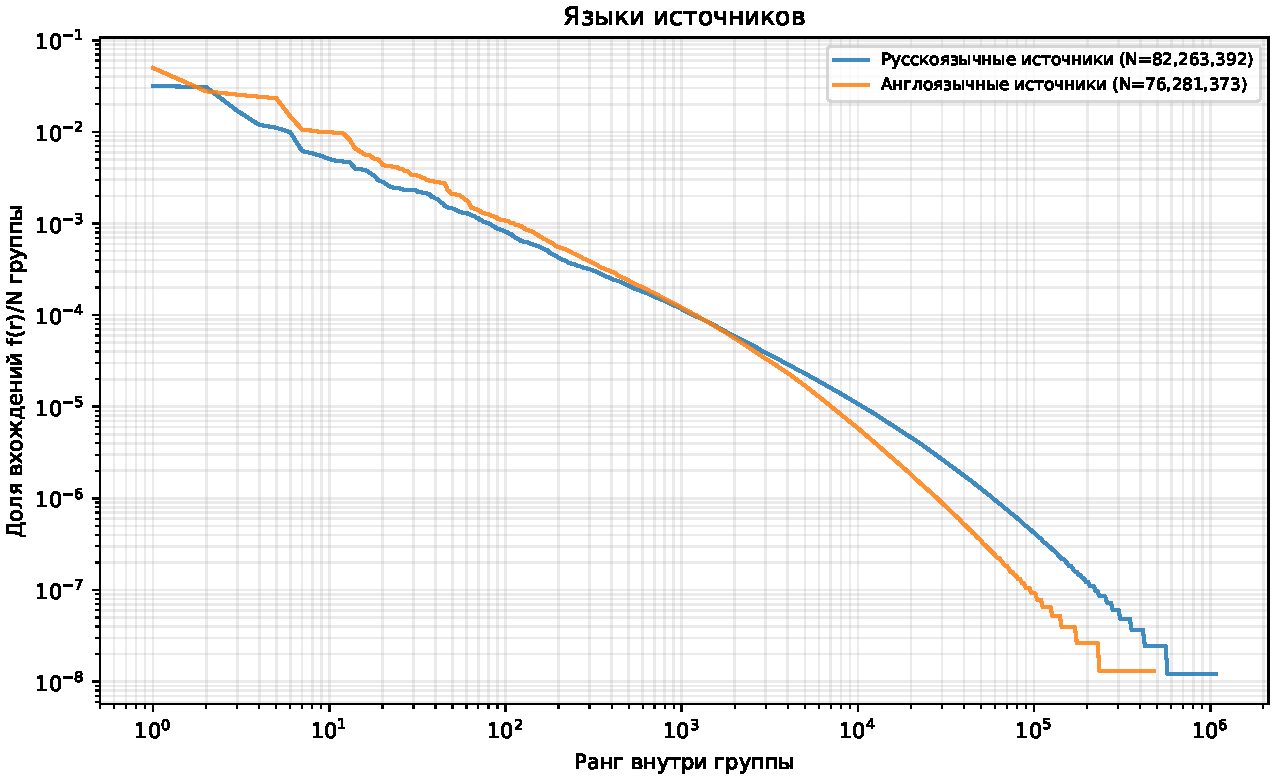
\includegraphics[width=\linewidth]{lab5/zipf_language.pdf}
\caption{Распределения русскоязычных и англоязычных источников}
\end{figure}

У русскоязычных источников степень на выбранном интервале около \ZipfRuAlpha{},
у англоязычных --- \ZipfEnAlpha{}. Русский словарь в этом снимке также больше.
Морфологическое разнообразие русского языка может вносить вклад, но
этот эксперимент не отделяет его от размера групп, состава сайтов,
собственных имён и структуры публикаций. Общая смесь языков даёт
свой показатель; переносить его на каждый язык отдельно нельзя.

\begin{figure}[H]
\centering
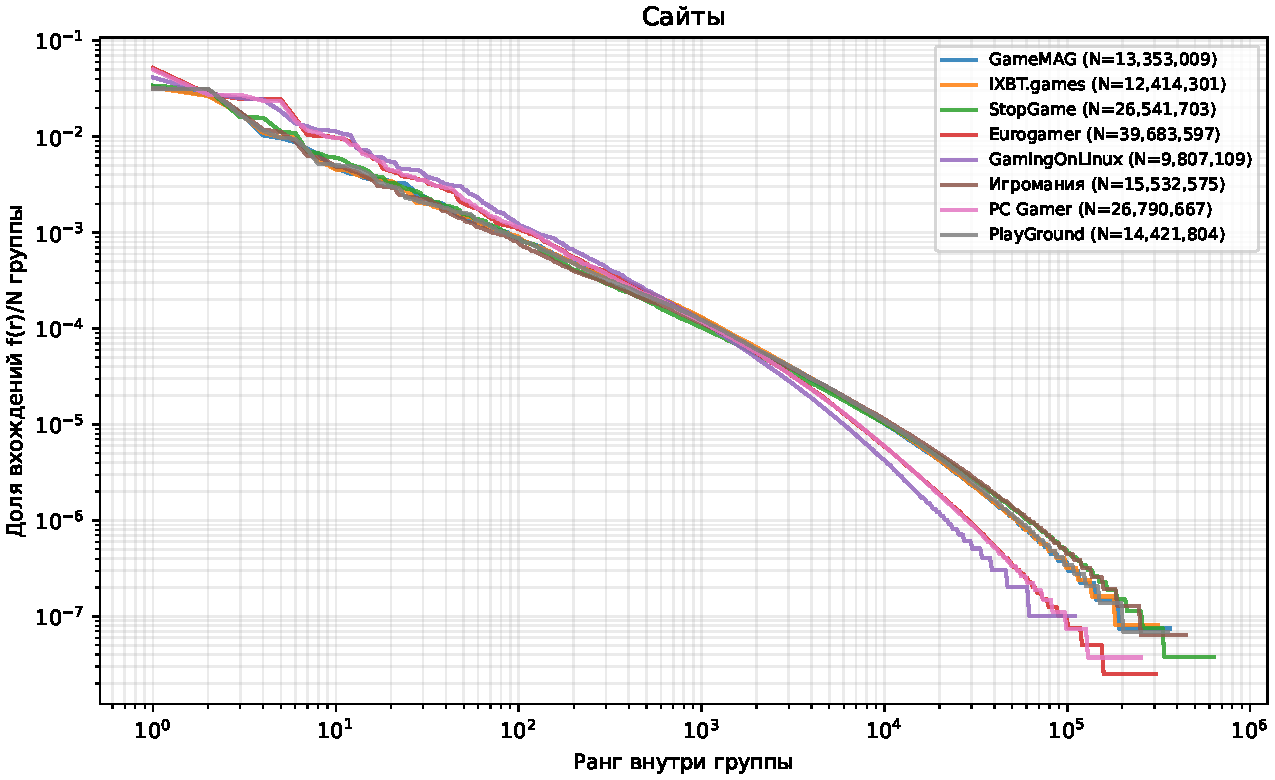
\includegraphics[width=\linewidth]{lab5/zipf_source.pdf}
\caption{Сравнение сайтов после нормировки частот внутри источника}
\end{figure}

Причины отклонения от идеальной модели --- конечный размер корпуса,
ограниченная игровая тематика, смесь языков, словоформы, собственные имена
и разная длина документов. Сам график не исключает влияния дублей или
ошибок парсинга и не оценивает качество поисковой выдачи.

\subsection{Программная реализация}
Подсчёт частот, ранжирование и подбор показателя степени выполнены
на C++. Python используется для подготовки данных и построения графиков.
Статистические показатели рассчитаны по всем терминам; на рисунках
используется логарифмическая выборка точек распределения.
Инструкция сборки и запуска приведена в \path{doc/lab5_run.md}.
Исходный код лабораторной работы:
\href{https://github.com/kirbasss/MAI-IR/tree/lab5}{github.com/kirbasss/MAI-IR/tree/lab5}.
\begin{figure}[H]
\centering
\begingroup
\hypersetup{urlcolor=black}
\qrcode[height=28mm]{https://github.com/kirbasss/MAI-IR/tree/lab5}
\endgroup
\caption{Ссылка на ветку лабораторной работы №5}
\end{figure}

\section{Вывод}
В работе построены частотные распределения словоформ игрового корпуса
и выполнено сравнение с законом Ципфа. На рангах
\ZipfFitMin{}--\ZipfFitMax{} общий показатель $\alpha=\ZipfAlpha{}$
близок к единице. Основные отклонения наблюдаются среди наиболее частых
терминов и в редком хвосте. Однократные термины составляют
\ZipfHapaxPercent{}\% словаря.

Сравнение групп показало различия между русскоязычными и англоязычными
источниками.
На результаты влияют состав корпуса, морфологическое разнообразие,
собственные имена и объём выборки. Поэтому закон Ципфа описывает
общую тенденцию, но не задаёт точные частоты отдельных слов.

Для информационного поиска полученное распределение показывает
сочетание небольшого числа частых терминов и большого числа редких,
расширяющих словарь. Это необходимо учитывать при выборе структуры
словаря и способов хранения индекса. Длины списков документов зависят
от документных частот и требуют отдельного подсчёта.
\end{document}
